\documentclass[12pt,a4paper]{article}
\usepackage[utf8]{inputenc}
\usepackage{amsmath,amssymb,amsthm}
\usepackage{graphicx}
\usepackage{hyperref}
\usepackage{booktabs}
\usepackage{xcolor}
\usepackage{listings}
\usepackage{geometry}
\usepackage{fancyhdr}
\usepackage{tikz}
\usepackage{longtable}
\usetikzlibrary{arrows.meta,shapes,positioning,calc}

\geometry{margin=1in}
\hypersetup{
    colorlinks=true,
    linkcolor=blue,
    urlcolor=blue,
    citecolor=blue
}

\pagestyle{fancy}
\fancyhf{}
\rhead{Lux Network}
\lhead{Tokenomics Whitepaper}
\rfoot{Page \thepage}

\definecolor{luxblue}{RGB}{0,100,200}
\definecolor{luxgold}{RGB}{218,165,32}

\title{\textbf{Lux Network Tokenomics}\\[1em]
\large A Comprehensive Framework for Deflationary Economics,\\ve-Governance, and Validator Incentives}
\author{Lux Industries\\
\texttt{https://lux.network}}
\date{Version 2.0 -- December 2025}

\begin{document}

\maketitle
\thispagestyle{empty}

\begin{abstract}
LUX is a \textbf{deflationary coin} used to pay for transactions on Lux Network. No more LUX can ever be minted---\textbf{half of every transaction fee is burned}. This whitepaper presents the complete tokenomics of the Lux Network, including token distribution, validator tiers, NFT membership passes, liquidity provider rewards, and the vote-escrowed governance system. With a fixed supply of 2 trillion tokens and a launch price of \$0.0001, Lux creates sustainable long-term alignment between validators, stakers, and the broader ecosystem.
\end{abstract}

\tableofcontents
\newpage

%==============================================================================
\section{Introduction}
%==============================================================================

\subsection{The Lux Network Vision}

The Lux Network is a next-generation Layer-1 blockchain designed for high performance, post-quantum security, and sustainable economic design. Central to Lux's architecture is a \textbf{deflationary tokenomics model} where half of all transaction fees are permanently burned.

\subsection{Key Economic Properties}

\begin{itemize}
    \item \textbf{Fixed Supply}: 2,000,000,000,000 LUX (2 trillion) --- no additional minting possible
    \item \textbf{Deflationary}: 50\% of all transaction fees are burned
    \item \textbf{Launch Price}: \$0.0001 USD per LUX
    \item \textbf{Fully Diluted Valuation}: \$220,000,000 at launch
    \item \textbf{Community Governance}: DAO controls 50\% of total supply
\end{itemize}

%==============================================================================
\section{Token Distribution}
%==============================================================================

\subsection{Total Supply}

The LUX token has a fixed total supply of \textbf{2 trillion tokens} (2,000,000,000,000 LUX). This supply is fully minted at genesis and can never be increased.

\subsection{Initial Allocation}

\begin{table}[h]
\centering
\begin{tabular}{lrrp{5cm}}
\toprule
\textbf{Category} & \textbf{\%} & \textbf{Tokens (LUX)} & \textbf{Notes} \\
\midrule
Lux DAO & 50\% & 1,000,000,000,000 & Locked, controlled by DAO \\
Public Sale & 20\% & 400,000,000,000 & 369 daily auctions, 10-20\% discount \\
Private Sale & 5\% & 100,000,000,000 & 25-50\% discount, 366d lock + 10\%/mo \\
Lux Team & 5\% & 100,000,000,000 & 366d lock + 10\%/mo release \\
Lux Developers & 5\% & 100,000,000,000 & 366d lock + 10\%/mo release \\
Network Treasury & 5\% & 100,000,000,000 & Market making \& liquidity only \\
Network Rewards & 5\% & 100,000,000,000 & Customer acquisition \\
Network Partners & 5\% & 100,000,000,000 & Partner incentives \\
\bottomrule
\end{tabular}
\caption{LUX Token Initial Distribution}
\label{tab:distribution}
\end{table}

\subsection{Key Metrics}

\begin{table}[h]
\centering
\begin{tabular}{lr}
\toprule
\textbf{Metric} & \textbf{Value} \\
\midrule
LUX Total Supply & 2,000,000,000,000 LUX \\
LUX Price (Launch) & \$0.0001 USD \\
Fully Diluted Valuation & \$220,000,000 USD \\
Available for Public Purchase & \$55,000,000 USD \\
\bottomrule
\end{tabular}
\caption{Token Metrics at Launch}
\label{tab:metrics}
\end{table}

\subsection{Vesting Schedules}

\textbf{Private Sale, Team, and Developers:}
\begin{itemize}
    \item 366 days initial lock from acquisition
    \item 10\% released monthly thereafter (10 months to full unlock)
\end{itemize}

\textbf{Public Sale:}
\begin{itemize}
    \item Not locked --- immediate liquidity
    \item 369 daily auctions spread over ~1 year
\end{itemize}

\textbf{Network Treasury, Rewards, Partners:}
\begin{itemize}
    \item Locked --- only used for designated purposes
    \item Requires DAO governance approval for any distribution
\end{itemize}

%==============================================================================
\section{Deflationary Mechanics}
%==============================================================================

\subsection{Fee Burning}

Unlike traditional blockchains, Lux implements aggressive deflation:

\begin{quote}
\textit{``Half of every transaction fee is burned permanently.''}
\end{quote}

\begin{equation}
\text{Burn Rate} = 0.5 \times \text{Total Transaction Fees}
\end{equation}

\subsection{Supply Reduction Over Time}

With consistent network usage, the circulating supply decreases:

\begin{equation}
\text{Supply}(t) = \text{Supply}_0 - \int_0^t 0.5 \times F(s) \, ds
\end{equation}

where $F(s)$ represents transaction fees collected at time $s$.

\subsection{Remaining Fee Distribution}

The 50\% of fees not burned are distributed via governance:

\begin{table}[h]
\centering
\begin{tabular}{lr}
\toprule
\textbf{Recipient} & \textbf{Default Weight} \\
\midrule
Validators & 48\% \\
DAO Treasury & 1\% \\
Protocol-Owned Liquidity & 1\% \\
\bottomrule
\end{tabular}
\caption{Distribution of Non-Burned Fees}
\label{tab:feedist}
\end{table}

%==============================================================================
\section{Validator Economics}
%==============================================================================

\subsection{Validator Tiers}

Lux supports multiple validator tiers to enable broad participation while maintaining network security:

\begin{table}[h]
\centering
\begin{tabular}{lrrrr}
\toprule
\textbf{Tier} & \textbf{USD Value} & \textbf{LUX Required} & \textbf{Max Count} \\
\midrule
Genesis Validator & \$1,000,000 & 1,000,000,000 & 100 \\
Validator & \$100,000 & 100,000,000 & 1,000 \\
Mini Validator & \$10,000 & 10,000,000 & 10,000 \\
Nano Validator & \$1,000 & 1,000,000 & 100,000 \\
\bottomrule
\end{tabular}
\caption{Validator Tiers and Requirements}
\label{tab:validators}
\end{table}

\subsection{Validator Counts Summary}

\begin{table}[h]
\centering
\begin{tabular}{lrr}
\toprule
\textbf{Category} & \textbf{LUX Allocation} & \textbf{Validator Count} \\
\midrule
Genesis (1B each) & 100,000,000,000 & 100 \\
Standard (100M each) & 100,000,000,000 & 1,000 \\
Mini (10M each) & 100,000,000,000 & 10,000 \\
Nano (1M each) & 100,000,000,000 & 100,000 \\
\midrule
\textbf{Total Validators} & \textbf{400,000,000,000} & \textbf{111,100} \\
\bottomrule
\end{tabular}
\caption{Validator Network Distribution}
\label{tab:validatorcount}
\end{table}

%==============================================================================
\section{NFT System}
%==============================================================================

\subsection{NFT Types}

Lux offers three NFT types, each with matching tiers aligned to validator economics:

\begin{enumerate}
    \item \textbf{Validator NFTs}: Represent validator positions with permanently locked LUX
    \item \textbf{Card NFTs}: Membership cards with network benefits and governance rights
    \item \textbf{Coin NFTs}: Collectible coins representing network participation
\end{enumerate}

\subsection{NFT Tiers}

All three NFT types share the same tier structure:

\begin{table}[h]
\centering
\begin{tabular}{lrrr}
\toprule
\textbf{Tier} & \textbf{USD Value} & \textbf{LUX Locked} & \textbf{Max Supply} \\
\midrule
Genesis & \$1,000,000 & 1,000,000,000 & 100 \\
Validator & \$100,000 & 100,000,000 & 1,000 \\
Mini & \$10,000 & 10,000,000 & 10,000 \\
Nano & \$1,000 & 1,000,000 & 100,000 \\
\bottomrule
\end{tabular}
\caption{Unified NFT Tier Structure}
\label{tab:nfttiers}
\end{table}

\subsection{Ethereum Genesis Collection}

The original Lux Genesis NFT collection was minted on Ethereum at:
\begin{verbatim}
0x31e0f919c67cedd2bc3e294340dc900735810311
\end{verbatim}

\textbf{Migration Rules:}
\begin{itemize}
    \item \textbf{Total Supply}: 50 NFTs (47 existing, 3 non-existent)
    \item \textbf{Test NFTs (IDs 1-13)}: Assigned to treasury (0x9011...)
    \item \textbf{Genesis NFTs (IDs 14-49)}: Minted to current Ethereum holders
    \item \textbf{LUX Locking}: Each NFT has 1 billion LUX permanently locked
\end{itemize}

\subsection{Permanent LUX Locking}

Genesis NFTs have a unique economic property:

\begin{quote}
\textit{``The LUX backing each Genesis NFT can NEVER be unlocked.''}
\end{quote}

\begin{itemize}
    \item \textbf{1B LUX per NFT}: Permanently locked in the NFT contract
    \item \textbf{Staking Rewards}: Flow to the current NFT holder
    \item \textbf{Claimable}: Holders can claim rewards via \texttt{claimRewards()}
    \item \textbf{Transferable}: NFT can be sold/transferred; new holder receives future rewards
    \item \textbf{Total Locked}: 47B LUX across all Genesis NFTs
\end{itemize}

\subsection{NFT Holder Benefits}

\begin{table}[h]
\centering
\begin{tabular}{lp{8cm}}
\toprule
\textbf{Tier} & \textbf{Benefits} \\
\midrule
Genesis & Premium validator priority, 10x governance multiplier, exclusive events, highest staking rewards \\
Validator & Validator queue priority, 5x DAO voting boost, early access to features \\
Mini & Reduced transaction fees, staking bonuses, premium support \\
Nano & Community access, basic staking rewards, network participation \\
\bottomrule
\end{tabular}
\caption{NFT Tier Benefits}
\label{tab:nftbenefits}
\end{table}

%==============================================================================
\section{Staking Rewards}
%==============================================================================

\subsection{Liquidity Provider Rewards}

LP rewards incentivize deep liquidity pools:

\begin{table}[h]
\centering
\begin{tabular}{lr}
\toprule
\textbf{Lock Duration} & \textbf{APY} \\
\midrule
1 month & 5\% \\
3 months & 20\% \\
6 months & 50\% \\
12 months & 111\% \\
\bottomrule
\end{tabular}
\caption{Liquidity Provider Reward Rates}
\label{tab:lprewards}
\end{table}

\textit{Note: Liquidity Rewards are paid at the end of the period in a lump sum. Users have a toggle option to automatically compound staked tokens to the next period. Rates are estimates based on pool rewards allocation.}

\subsection{Single-Sided Staking}

Single-sided staking allows LUX holders to earn yield without impermanent loss:

\begin{table}[h]
\centering
\begin{tabular}{lr}
\toprule
\textbf{Lock Duration} & \textbf{APY} \\
\midrule
1 month & 1\% \\
3 months & 4\% \\
6 months & 10\% \\
12 months & 25\% \\
\bottomrule
\end{tabular}
\caption{Single-Sided Staking Rates}
\label{tab:singlestaking}
\end{table}

\subsection{Staking vs LP Comparison}

\begin{center}
\begin{tikzpicture}[scale=0.8]
    \draw[->] (0,0) -- (14,0) node[right] {Lock Duration};
    \draw[->] (0,0) -- (0,6) node[above] {APY \%};
    
    % LP rewards line
    \draw[thick,luxblue] (0,0.25) -- (3,1) -- (7,2.5) -- (14,5.55);
    \node[luxblue,right] at (14,5.55) {\small LP (111\%)};
    
    % Single-sided line
    \draw[thick,luxgold] (0,0.05) -- (3,0.2) -- (7,0.5) -- (14,1.25);
    \node[luxgold,right] at (14,1.25) {\small Single (25\%)};
    
    % X-axis labels
    \draw (0,-0.1) -- (0,0.1) node[below=0.2cm] {\small 0};
    \draw (3,-0.1) -- (3,0.1) node[below=0.2cm] {\small 1mo};
    \draw (7,-0.1) -- (7,0.1) node[below=0.2cm] {\small 6mo};
    \draw (14,-0.1) -- (14,0.1) node[below=0.2cm] {\small 12mo};
\end{tikzpicture}
\end{center}

%==============================================================================
\section{Vote-Escrowed Tokenomics (vLUX)}
%==============================================================================

\subsection{Lock Mechanism}

The vLUX system enables token holders to lock LUX for a period between 1 week and 4 years, receiving non-transferable voting power in return.

\begin{equation}
\text{vLUX}(t) = \text{LUX}_{\text{locked}} \times \frac{t_{\text{end}} - t_{\text{current}}}{\text{MAX\_LOCK}}
\end{equation}

where:
\begin{itemize}
    \item $\text{LUX}_{\text{locked}}$: Amount of LUX locked
    \item $t_{\text{end}}$: Lock expiration timestamp
    \item $\text{MAX\_LOCK}$: Maximum lock duration (4 years = 126,144,000 seconds)
\end{itemize}

\subsection{Voting Power Decay}

Voting power decays linearly over time:

\begin{center}
\begin{tikzpicture}[scale=0.9]
    \draw[->] (0,0) -- (10,0) node[right] {Time};
    \draw[->] (0,0) -- (0,5) node[above] {vLUX};
    \draw[thick,luxblue] (0,4) -- (8,0);
    \draw[dashed] (0,4) -- (-0.3,4) node[left] {1000 vLUX};
    \draw[dashed] (8,0) -- (8,-0.3) node[below] {4 years};
    \draw[dashed] (4,2) -- (4,-0.3) node[below] {2 years};
    \draw[dashed] (4,2) -- (-0.3,2) node[left] {500 vLUX};
    \fill[luxblue] (0,4) circle (2pt);
    \fill[luxblue] (4,2) circle (2pt);
    \fill[luxblue] (8,0) circle (2pt);
    \node[above right] at (1,3.5) {\small Lock 1000 LUX for 4 years};
\end{tikzpicture}
\end{center}

\subsection{Gauge Voting}

vLUX holders vote on gauge weights to direct fee distribution:

\begin{table}[h]
\centering
\begin{tabular}{lrp{7cm}}
\toprule
\textbf{Gauge} & \textbf{Default Weight} & \textbf{Purpose} \\
\midrule
Burn & 50\% & Deflationary pressure via token destruction \\
Validators & 48\% & Validator and delegator rewards \\
DAO Treasury & 1\% & Governance and development funding \\
Protocol Liquidity & 1\% & DEX liquidity provision \\
\bottomrule
\end{tabular}
\caption{Default Fee Distribution Gauges}
\label{tab:gauges}
\end{table}

%==============================================================================
\section{Staked LUX (sLUX)}
%==============================================================================

\subsection{Overview}

sLUX is a liquid staking token representing staked LUX plus accrued yield. Unlike vLUX (governance), sLUX is transferable and can be used as collateral in DeFi protocols.

\subsection{Exchange Rate}

The sLUX exchange rate increases over time as rewards accrue:

\begin{equation}
\text{ExchangeRate} = \frac{\text{TotalLUX} + \text{AccruedRewards}}{\text{TotalSupply}_{\text{sLUX}}}
\end{equation}

\subsection{Cooldown Period}

\begin{itemize}
    \item \textbf{Stake}: Deposit LUX, receive sLUX at current exchange rate
    \item \textbf{Unstake}: Start 7-day cooldown, then withdraw
\end{itemize}

%==============================================================================
\section{Synthetic Assets}
%==============================================================================

\subsection{The Synth Protocol}

Lux features an Alchemix-style synthetic asset protocol:
\begin{enumerate}
    \item Deposit yield-bearing collateral (e.g., sLUX, yvWETH)
    \item Mint synthetic assets (sUSD, sETH, sBTC, sLUX)
    \item Debt self-repays as collateral accrues yield
\end{enumerate}

\subsection{Supported Synths}

\begin{itemize}
    \item \textbf{sUSD}: Synthetic USD, pegged to \$1
    \item \textbf{sETH}: Synthetic Ethereum
    \item \textbf{sBTC}: Synthetic Bitcoin
    \item \textbf{sLUX}: Synthetic LUX (leveraged exposure)
    \item \textbf{sSOL}: Synthetic Solana
    \item \textbf{sTON}: Synthetic Toncoin
    \item \textbf{sADA}: Synthetic Cardano
    \item \textbf{sAVAX}: Synthetic Avalanche
    \item \textbf{sBNB}: Synthetic Binance Coin
    \item \textbf{sPOL}: Synthetic Polygon
    \item \textbf{sZOO}: Synthetic Zoo Token
    \item \textbf{sAI}: Synthetic AI Token
\end{itemize}

%==============================================================================
\section{Smart Contract Architecture}
%==============================================================================

\subsection{Core Contracts}

\begin{table}[h]
\centering
\begin{tabular}{ll}
\toprule
\textbf{Contract} & \textbf{Purpose} \\
\midrule
\texttt{WLUX} & Wrapped LUX (ERC20) \\
\texttt{vLUX} & Vote-escrowed LUX \\
\texttt{GaugeController} & Gauge weight voting \\
\texttt{FeeSplitter} & Protocol fee distribution \\
\texttt{ValidatorVault} & Validator/delegator economics \\
\texttt{sLUX} & Liquid staking token \\
\texttt{SynthFeeSplitter} & Synth protocol fees \\
\bottomrule
\end{tabular}
\caption{Core Smart Contracts}
\label{tab:contracts}
\end{table}

\subsection{Contract Interactions}

\begin{center}
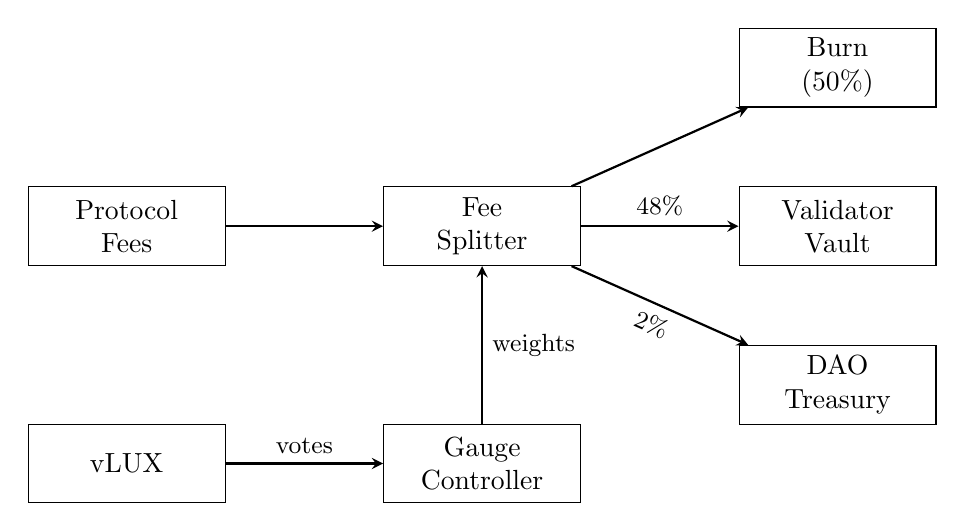
\begin{tikzpicture}[
    node distance=2cm,
    box/.style={rectangle, draw, minimum width=2.5cm, minimum height=1cm, align=center},
    arrow/.style={->, >=stealth, thick}
]
    \node[box] (protocol) {Protocol\\Fees};
    \node[box, right=of protocol] (splitter) {Fee\\Splitter};
    \node[box, above right=1cm and 2cm of splitter] (burn) {Burn\\(50\%)};
    \node[box, right=of splitter] (validator) {Validator\\Vault};
    \node[box, below right=1cm and 2cm of splitter] (dao) {DAO\\Treasury};
    \node[box, below=of splitter] (gauge) {Gauge\\Controller};
    \node[box, left=of gauge] (vlux) {vLUX};

    \draw[arrow] (protocol) -- (splitter);
    \draw[arrow] (splitter) -- (burn);
    \draw[arrow] (splitter) -- (validator) node[midway,above] {\small 48\%};
    \draw[arrow] (splitter) -- (dao) node[midway,below,sloped] {\small 2\%};
    \draw[arrow] (gauge) -- (splitter) node[midway,right] {\small weights};
    \draw[arrow] (vlux) -- (gauge) node[midway,above] {\small votes};
\end{tikzpicture}
\end{center}

%==============================================================================
\section{Security Considerations}
%==============================================================================

\subsection{Economic Security}

\begin{itemize}
    \item \textbf{Vote Delay}: 10-day delay between votes prevents manipulation
    \item \textbf{Flash Loan Protection}: vLUX requires time-locked LUX
    \item \textbf{Weekly Epochs}: Gauge weights update weekly only
\end{itemize}

\subsection{Slashing Protection}

The ValidatorVault maintains a 5\% slashing reserve to protect delegators from validator misbehavior.

%==============================================================================
\section{Governance and DAO}
%==============================================================================

\subsection{DAO Structure}

The Lux DAO controls the 50\% treasury allocation (1 trillion LUX) and can:
\begin{itemize}
    \item Add/remove gauges
    \item Adjust fee splitter parameters
    \item Fund development initiatives
    \item Manage protocol-owned liquidity
\end{itemize}

\subsection{SubDAOs}

\begin{itemize}
    \item \textbf{Grants DAO}: Developer funding
    \item \textbf{Security DAO}: Audit coordination
    \item \textbf{Validator DAO}: Validator set management
    \item \textbf{Treasury DAO}: Investment strategy
\end{itemize}

%==============================================================================
\section{Conclusion}
%==============================================================================

The LUX tokenomics system creates a sustainable deflationary ecosystem:

\begin{itemize}
    \item \textbf{Fixed Supply}: 2 trillion LUX, no inflation possible
    \item \textbf{Aggressive Deflation}: 50\% of all fees burned
    \item \textbf{Aligned Incentives}: Validators, stakers, and DAO share remaining fees
    \item \textbf{Tiered Access}: Four tiers from \$1K nano to \$1M genesis
    \item \textbf{Genesis NFTs}: Permanent LUX locking with staking rewards to holders
    \item \textbf{High Yield}: Up to 111\% APY for liquidity providers
    \item \textbf{Community Governance}: vLUX holders control fee distribution
\end{itemize}

As network usage grows, deflation accelerates while remaining fees fund validators and development. This creates a virtuous cycle where increased adoption benefits all stakeholders.

%==============================================================================
\appendix
\section{Appendix: Token Summary}
%==============================================================================

\begin{table}[h]
\centering
\begin{tabular}{lr}
\toprule
\textbf{Parameter} & \textbf{Value} \\
\midrule
Total Supply & 2,000,000,000,000 LUX \\
Launch Price & \$0.0001 USD \\
FDV at Launch & \$220,000,000 USD \\
Burn Rate & 50\% of transaction fees \\
Max Validators & 111,100 \\
Max Lock Period & 4 years \\
Cooldown Period & 7 days \\
Vote Delay & 10 days \\
\bottomrule
\end{tabular}
\caption{LUX Token Summary}
\end{table}

%==============================================================================
\section{Appendix: References}
%==============================================================================

\begin{enumerate}
    \item Curve Finance. ``Vote-Escrowed CRV.'' \url{https://curve.fi}
    \item Alchemix. ``Self-Repaying Loans.'' \url{https://alchemix.fi}
    \item Lido Finance. ``Liquid Staking.'' \url{https://lido.fi}
    \item Lux Network. ``Technical Documentation.'' \url{https://docs.lux.network}
\end{enumerate}

\end{document}
